\chapter{Development}
\label{ch:dev}

\begin{chapterquote}{Nils Bohr}
	"Prediction is very difficult, especially if it's about the future."
\end{chapterquote}
In this section we will explain the data used for the experiments, the process of preprocessing, and the experiments for each model. First, we present the parameter selection experiments. Then, we explain the experiments for stock market price prediction as well as the metrics and criteria used to compare the models.

\section{Data description}
The data used in this study includes the closure stock market prices of \textit{Wal-Mart de México, S.A.B. de C.V.} known as WALMEX. The data was extracted from Yahoo! Finance applying a weekly filter over a time interval: from 02/01/2012 to 16/01/2017.

The result was a database with 264 weekly prices in MXN currency. The average price is \$32.72 MXN with a standard deviation of 4.32. The minimum price is \$28.09 MXN and the maximum is \$47.22 MXN. Figure \ref{fig:walmexFreq} shows the frequency of the prices by intervals since the data is too variable to be analyzed by the frequency of each price. It can be seen that the interval of highest frequency includes the prices between \$34.5 to \$35.4. 

On the other hand, if we analyze the prices by the average price of each month and year it can be noticed that the years can be classified in four different intervals. Nevertheless, there are no two consecutive years that kept the same average price interval. In 2014 the lowest average price was registered and the highest appears in 2016.

When analyzing by month it can be seen in Figure \ref{fig:walmexMonth} that the months can be grouped in three intervals. In this case, there are following months that remain in the same interval: from May to July and from August to September. 

 
\begin{figure}
\center
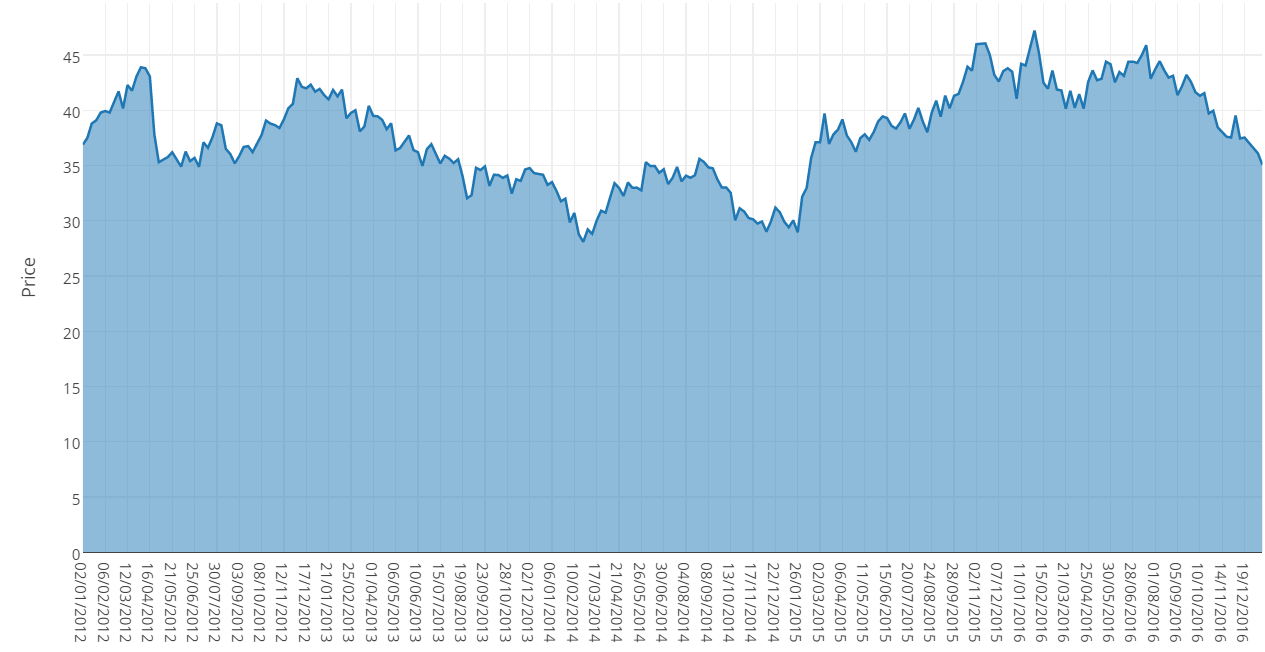
\includegraphics[width=12.5cm,height=5.5cm]{Figures/wamexCompleto.PNG}
\caption{Weekly WALMEX Stock Prices}
\label{fig:walmexComp}
\end{figure}

\begin{figure}
\center
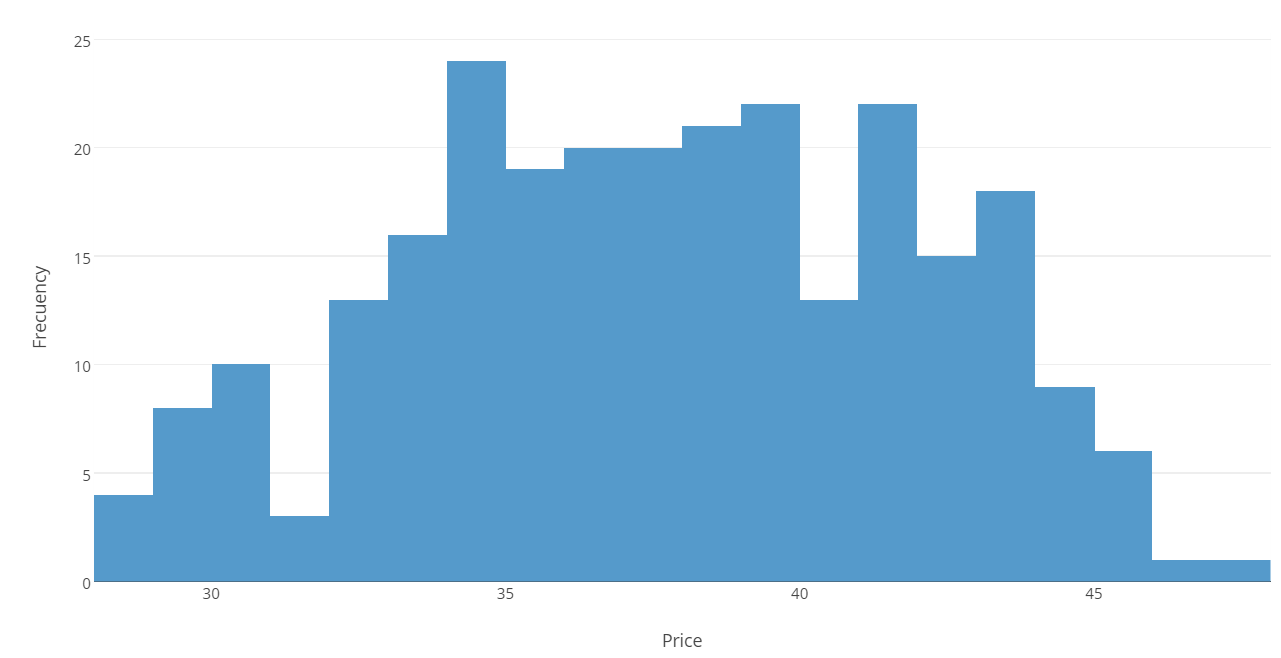
\includegraphics[width=13.5cm,height=6.5cm]{Figures/walmexHistogram.PNG}
\caption{Frequency of Prices by Intervals}
\label{fig:walmexFreq}
\end{figure}

\begin{figure}
\center
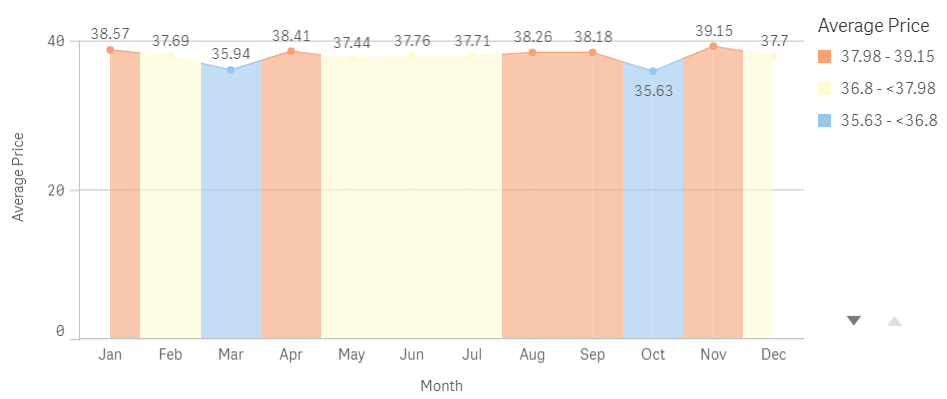
\includegraphics[width=14.5cm,height=6.5cm]{Figures/walmexMonth.PNG}
\caption{Monthly Average Stock Price}
\label{fig:walmexMonth}
\end{figure}

\begin{figure}
\center
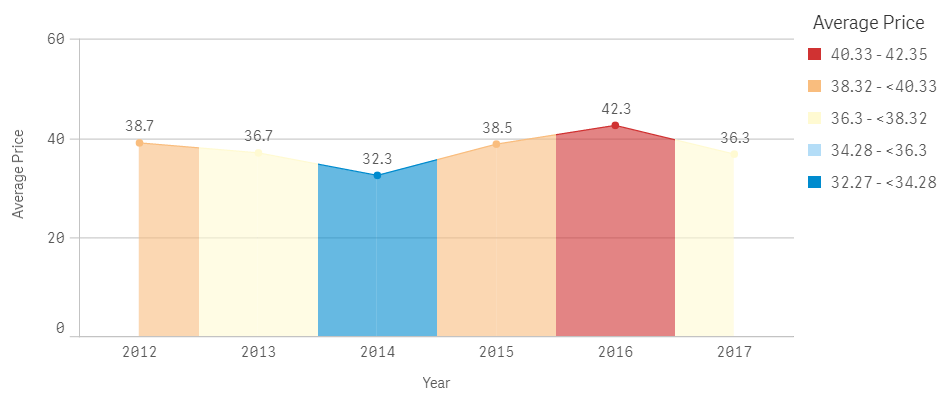
\includegraphics[width=14.5cm,height=6.5cm]{Figures/walmexYear.PNG}
\caption{Yearly Average Stock Price}
\label{fig:walmexYear}
\end{figure}

\section{Preprocessing}
In this section we explain how prices are mapped to an adequate representation that the three models understand. The three models proposed belong to supervised learning. Hence, data needs to be vectorized and target values need to be defined. The preprocessing took in account three steps:

\begin{enumerate}
\item Data split
\item Normalization
\item Vectorization
\end{enumerate}

First, the database was divided in two subsets: 67\% of the data for training and the remaining 33\% for testing. Since we are working with time series, the order of the values was respected. Therefore, the first 177 prices were assigned to the training subset and the last 88 values to the testing subset. From this point, the testing subset was not occupied until the evaluation phase.

The next step was to normalize the data, meaning, the data was rescaled to the interval $[0,1]$ as follows:

\begin{equation}
\label{eq:normalize}
x_{new}=\frac{x-x_{min}}{x_{max}-x_{min}}
\end{equation}

where $x_{min}$ is the minimum value in the training subset and $x_{max}$ is the maximum value in the training subset. 

For the evaluation phase, the testing subset was also normalized taking in account the maximum and minimum value of the training subset in order to avoid adding future information to the testing subset.

In this work, sequences of three prices were defined as the attributes of the database. Hence, the target value is the fourth one in the sequence. Since the data is already in weekly time intervals, there is no need to keep the dates for each price.

This representation gave us a training set of 173 examples and a testing set of 84. The first five examples of prive vectors with its target price are shown in table \ref{table:trainPrices}. Table \ref{table:train} exhibits the vectors after normalization.


\begin{table}{}
\begin{center}
\begin{tabular}{ c | c | c | c }
    \hline
     \textbf{Price 1} &  \textbf{Price 2} &    \textbf{Price 3} &   \textbf{TargetPrice}\\ \hline
    36.88&  37.49&  38.79 &39.09\\ \hline
    37.49&  38.79&  39.09&39.79\\ \hline
    38.79&  39.09&  39.79&39.93\\ \hline
   39.09&  39.79&  39.93&39.79\\ \hline
    39.79&  39.93&  39.790&40.72\\ \hline
    \hline
  \end{tabular}
\caption{First 5 Examples of Price Vectors}
 \label{table:trainPrices}
\end{center}

 \end{table}


\begin{table}{}
\begin{center}
\begin{tabular}{ c | c | c | c }
    \hline
    \textbf{Price 1} &  \textbf{Price 2} &    \textbf{Price 3} &   \textbf{Target Price} \\ \hline
    0.55696201 &  0.59493685&  0.6778481 &0.69620258\\ \hline
    0.59493685 &  0.6778481 &  0.69620258 &0.74050641\\ \hline
     0.6778481 &  0.69620258 &  0.74050641&0.74936712\\ \hline
     0.69620258 & 0.74050641 &  0.74936712 &0.74050641\\ \hline
     0.74050641 &  0.74936712 &  0.74050641 &0.79936719\\ \hline
    \hline
  \end{tabular}
\caption{Price Vectors after Normalization}
\end{center}
\label{table:train}
 \end{table}
 
 \section{Methodology}
 %\label{ch:methodology}

%\begin{chapterquote}{Ludwig Wittgenstein}
%	The limits of my language mean the limits of my world.
%\end{chapterquote}
The three models were implemented in Anaconda with Python 2.7.12 in a 64 bits latop with 4GB of RAM. The processor of the system is Intel(R) Core(TM) i5-3337U CPU @ 1.80 GHz and the operative system is Windows 10. In order to replicate the experimental results we fixed the seed to 14. 
\subsection{Parameter Selection}

Each model required a parameter to be chosen. For the ANN we looked for the number of hidden layers, for the SVM the parameter to choose is the C; and for the RNN we looked for the number of LSTM cells required.

Since it is a time series problem, the order of the examples must be respected. To make sure this happens, the parameters were selected using time series cross-validation over the training subset. In this k-fold cross-validation variant, successive training sets are supersets of those that come before them. In all cases, we looked for the parameter that minimized the mean square error (MSE). 

For each cross validation the next steps were implemented:
\begin{enumerate}
\item Split the training data in $k=5$ arranged subsets
\item For each candidate parameter p:
\item  Build the model with p
\begin{enumerate}
\item For each split of $k-1=4$ length subsets:
\begin{enumerate}
\item Train the model
\item Evaluate the model using the left subset
\item Calculate and keep the MSE
\end{enumerate}
\item Calculate and keep the average and the standard deviation of the MSEs
\end{enumerate}
\item Choose the parameter with the minimum MSE
\end{enumerate}

\subsubsection{Artificial Neural Network}

The artificial neural model was implemented using Pybrain, a flexible machine learning library for Python. The input layer had three neurons for each real price and the output layer had only one neuron for the prediction of the next price. The minimum MSE after applying cross validation was gotten using three neurons in the hidden layer as shown in  Figure \ref{fig:cvNN}

\begin{figure}[h]
\centering
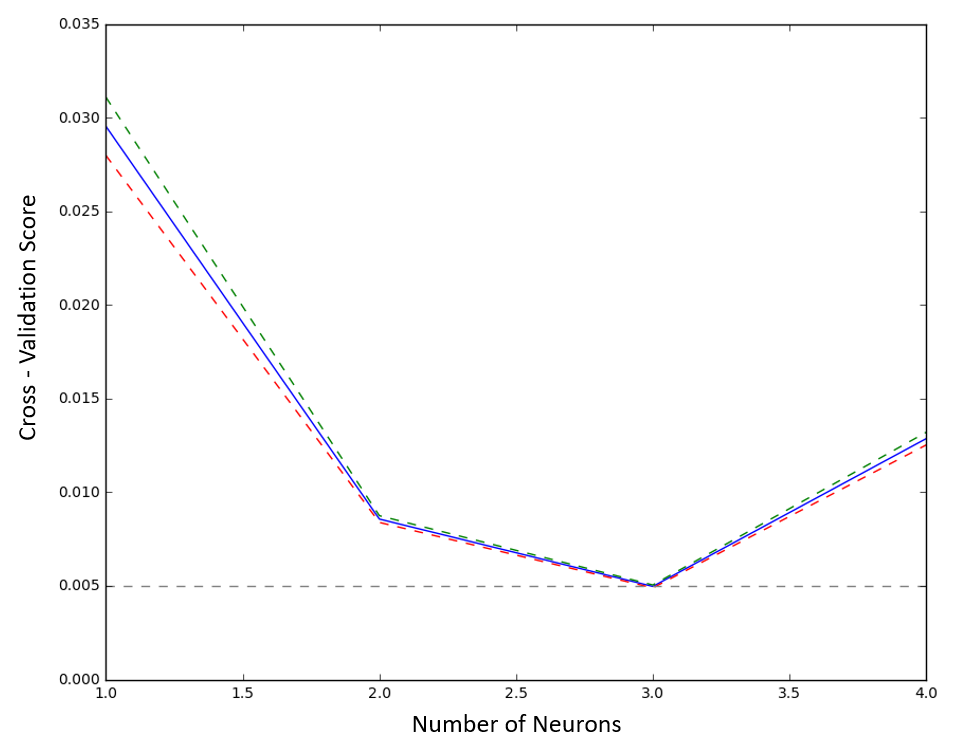
\includegraphics[width=10cm,height=6.5cm]{cvNN.PNG}
\caption{MSE for each ANN Configuration}
\begin{minipage}{12cm}
    \footnotesize
    \emph \\ The blue line shows the average of the MSEs of each network configuration. The green and the red lines represent the error lines showing the +/- standard deviation errors of the scores
    \end{minipage}
\label{fig:cvNN}
\end{figure}

\subsubsection{Support Vector Machine}
The support vector machine was implemented using the scikit-learn library of Python. It provides simple and efficient tools for data mining and data analysis. We used a sigmoid kernel and C=3 which got the minimum MSE as shown in Figure \ref{fig:cvSVM}

\begin{figure}[h]
\centering
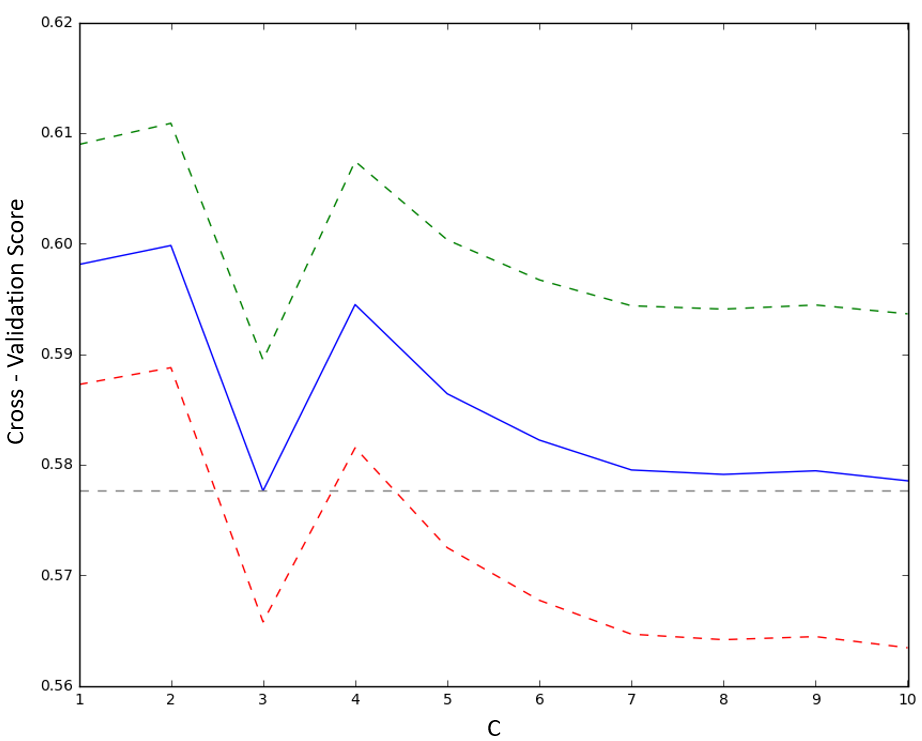
\includegraphics[width=10cm,height=6.5cm]{cvSVM.PNG}
\caption{MSE for each SVM Configuration}
\begin{minipage}{12cm}
    \footnotesize
    \emph \\ The blue line shows the average of the MSEs of each network configuration. The green and the red lines represent the error lines showing the +/- standard deviation errors of the scores
    \end{minipage}

\label{fig:cvSVM}
\end{figure}

\subsubsection{Recurrent Neural Network}

The model was implemented in Keras, a high-level neural network library written in Python. It can run on top of either TensorFlow or Theano and with CPU or GPU. It supports recurrent neural networks, and arbitrary connectivity schemes including multi-input and multi-output training. For this study we used Theano as background.

The model had an input, a hidden and an output layer. It had 3 outputs for each real price. The single hidden layer had 10 LSTM units with a drop out of 0.03 for the non-recurrent connections. 

Finally, we had a full connected layer with one output which refers to the prediction of the price. The network implements ADAM SGD optimizer to adapt the learning rate dynamically since the data is sparse. 

As shown in Figure \ref{fig:cvRNN}, the minimum MSE is not obtained with 10 LSTMs. Nevertheless, with one more LSTM the MSE is higher and then it drops again. Since the difference between the MSE with 10 LSTMs and with 16 LSTMs is just 0.003, we decided to use 10 LSTMs. In addition, using less LSTMs requires less parameters to be calculated by the network.  

\begin{figure}[h]
\centering
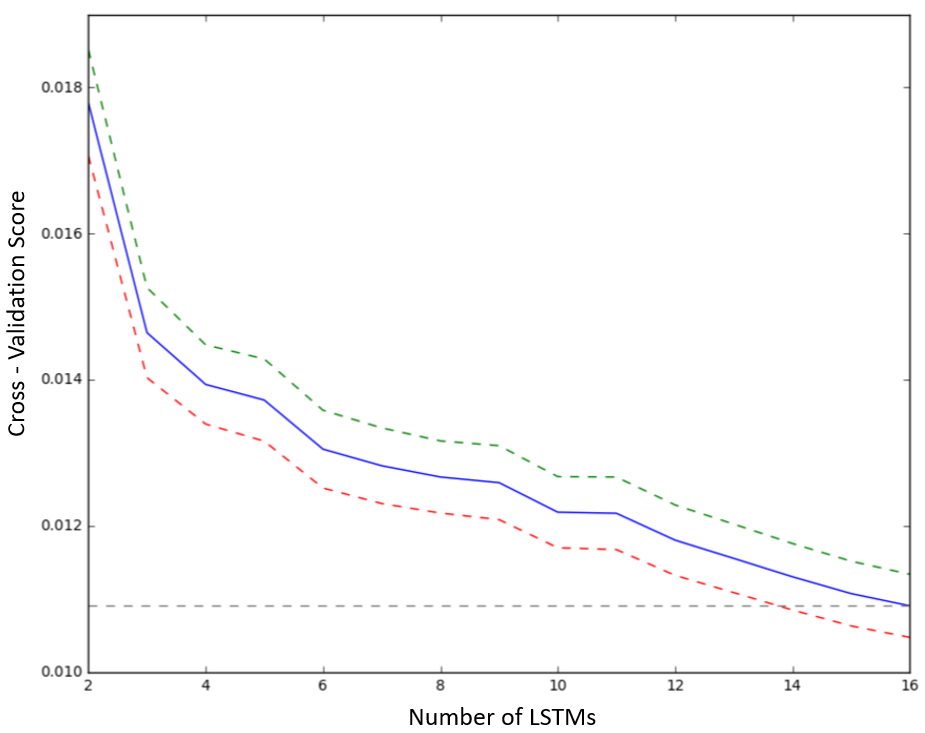
\includegraphics[width=10cm,height=6.5cm]{cvRNN.PNG}
\caption{MSE for each RNN Configuration}
\begin{minipage}{12cm}
    \footnotesize
    \emph \\ The blue line shows the average of the MSEs of each network configuration. The green and the red lines represent the error lines showing the +/- standard deviation errors of the scores
    \end{minipage}
\label{fig:cvRNN}
\end{figure}

\subsection{Comparison Criteria}

Since we are predicting stock market prices this study is strongly interested in two main criteria:

\begin{itemize}
\item How precise is the model to predict the price
\item How precise is the model to capture the up and down movements
\end{itemize}

For the first criteria we used the MSE to compare each model's performance. The second criteria required a new categoric vector for the real test values and for the predicted values of each model in order to express the ups and downs of the prices.

This vector mapped a 0 if the new price was lower than the past one and 1 if it was higher. In this way we could compare the models using the accuracy, precision, recall, and F1 scores. Another resource used is the confusion matrix. 

The metrics as well as the confusion matrix are explained as follows:

\begin{itemize}
\item \textbf{MSE:} the average of the quadratic differences between the real and the predicted value
\begin{equation}
MSE=\frac{1}{n}\sum_i (Y_{real}-Y_{predicted})^2
\label{eq:msemet}
\end{equation}
\item \textbf{Accuracy:} the proportion where the predicted values are the same as the real values out of the total of examples

\item \textbf{Precision:} the number of true positives divided by the sum of true positives and false positives, meaning, the total number of elements labeled as belonging to the positive class 
\begin{equation}
Precision=\frac{TP}{TP+TN}
\label{eq:precision}
\end{equation}
\item \textbf{Recall}: the number of true positives divided by the true positives plus the false negatives, meaning, the total number of elements that actually belong to the positive class
\begin{equation}
Recall=\frac{TP}{TP+FN}
\label{eq:recall}
\end{equation}
\item \textbf{F1 Score:} it is a weighted average of the precision and recall. The F1 score reaches its best value at 1 and worst at 0 and is equals to two times the division between the product of precision and recall, and the sum of both metrics.
\begin{equation}
F1 Score=2*\frac{Precision*Recall}{Precision+Recall}
\label{eq:fiscore}
\end{equation}
\item \textbf{Confusion Matrix:} it shows the true positive, true negative, false positive and false negative values. Each column represents the examples in a predicted class while each row represents the examples in an actual class.
\begin{center}
$Confusion$ $Matrix$$ = 
\left[ {\begin{array}{*{20}c}
   TP & FP  \\
   FN & TN  \\

 \end{array} } \right]
$
\end{center}

\end{itemize}


























 